\documentclass{article}
\usepackage{amsmath}

\usepackage{pgfplots}
\pgfplotsset{compat=1.15}
\usepackage{tkz-euclide}
\usetkzobj{all}

\usepackage{fancyhdr}
\usepackage[a4paper,left=1in,right=1in,top=1.5in,bottom=1in]{geometry} % Uncomment for narrow margins
\usepackage{parskip}
\usepackage{float}

\date{x/x/20xx}
\newcommand\addtag{\refstepcounter{equation}\tag{\theequation}}
\renewcommand*{\arraystretch}{1.5}


\begin{document}

\fancyhead[R]{Trigonometric identities}
\pagestyle{fancy}


\section{Basics}

In any equation with trigonometric functions, we usually try to treat $\sin$'s and $\cos$'s as the basic building blocks. Therefore we want to reduce an equation into something that only has $\sin$'s, or only has $\cos$'s.

Only use $\tan$ in special cases, such as when we have an equation like
\[
a\cos\theta=b\sin\theta\,,\qquad a,b\text{ constants}\,,
\]
or if we can turn the equation into only $\tan$'s.

When we have \emph{even} powers of $\sin$'s and $\cos$'s we can use
\[
\label{eqn:core}
\sin^2 x + \cos^2 x = 1 \addtag
\]
to transform everything into either $\sin$ or $\cos$. 

Divide \eqref{eqn:core} by $\cos^2x$ to get the equation relating $\tan$ and $\sec$
\[
\label{eqn:coretan}
\tan^2x+1 = \sec^2x \addtag
\]

Divide \eqref{eqn:core} by $\sin^2x$ to get the equation relating $\cot$ and $\mathrm{cosec}$
\[
\label{eqn:corecot}
1 + \cot^2x=\mathrm{cosec}^2x \addtag
\]
Use these to turn the $\tan$'s and $\cot$'s into $\cos$'s and $\sin$'s. Equations \eqref{eqn:core}, \eqref{eqn:coretan} and \eqref{eqn:corecot} are \textbf{not} given in the formula sheet and should definitely be remembered.

Some properties of $\sin$ and $\cos$:
\begin{itemize}
    \item $\sin(-x)=-\sin x$, $\cos(-x)=\cos x$. So $\tan(-x)=-\tan x$.
    \item $\sin$ and $\cos$ are periodic in $2\pi$. This means that $\sin(x+2\pi)=\sin x$. The $\tan$ is periodic in $\pi$.
    \item $\sin$ and $\cos$ are related by an offset of $\pi/2$. $\cos x = \sin(x+\pi/2)$. You can verify this using the angle addition formula.
    \[
    \sin\left(x+\frac{\pi}{2}\right) = \sin x\cos\left(\frac{\pi}{2}\right) + \cos x\sin\left(\frac{\pi}{2}\right) = \cos x
    \]
    You can also use the angle addition formula to verify that $\cos(\theta+\pi) = -\cos\theta$, and $\sin(\theta+\pi) = -\sin\theta$.
\end{itemize}

\textbf{Exact angles.} You should remember that there are exact results for the $\sin$, $\cos$ and $\tan$ of $30^\circ$, $45^\circ$ and $60^\circ$ angles, though most calculators will give you the results for these.
\[
\begin{array}{c|c|c|c}
    \theta & 30^\circ & 45^\circ & 60^\circ\\
    \hline
    \sin\theta & \frac{1}{2} & \frac{\sqrt{2}}{2} & \frac{\sqrt{3}}{2}\\
    \cos\theta & \frac{\sqrt{3}}{2} & \frac{\sqrt{2}}{2} & \frac{1}{2}
\end{array}
\]

The $\tan$ has a different set of values for these angles.
\[
\begin{array}{c|c|c|c}
    \theta & 30^\circ & 45^\circ & 60^\circ\\
    \hline
    \tan\theta & \frac{\sqrt{3}}{3} & 1 & \sqrt{3}
\end{array}
\]


\section{Inverses}

The inverse $f^{-1}$ of a function $f$ is defined such that $f^{-1}(f(x))=f(f^{-1}(x))=x$. This means that $\sin^{-1}(\sin(x))=x$, and also $\sin(\sin^{-1}(x))=x$.

The easiest way to find the value of an inverse trig function is by looking at the graph of the trig function. \textbf{Example.} if we want to find $\sin^{-1}(\sqrt{3}/2)$, this is the same as finding when $x$ gives $\sin x=\sqrt{3}/2$, so

\begin{figure}[H]
    \centering
    \begin{tikzpicture}[xscale=0.8, yscale=0.8]
    \begin{axis}[axis x line=middle, axis y line=middle, ymax=1.2, ymin=-1.2, xmax=600, xtick={0,60,180,360}, ytick={0.866}, yticklabel={$\sqrt{3}/2$}]
        \addplot[
        smooth,
        color=blue,
        domain=0:540,
        samples=100,
        ]{sin(x)};
        \addplot[
        color=red,
        domain=0:540,
        ]{sqrt(3)/2};
        \draw[dashed] (60,0) -- (60,0.866);
        \draw[dashed] (120,0.866) -- (120,0);
        \draw[dashed] (420,0) -- (420,0.866);
        \draw[dashed] (480,0) -- (480,0.866);
    \end{axis}
    \end{tikzpicture}
\end{figure}

Since the calculator gives $\sin^{-1}(\sqrt{3}/2)=60^\circ$, the next time $\sin(x)=\sqrt{3}/2$ is when the curve comes back down at $(90-60)+90 = 120^\circ$. Following that, we have the next angle at $360+60 = 420^\circ$, and $360+120=480^\circ$.

\textbf{Another example:} $\cos^{-1}(-0.8)$. The calculator gives the closest value, $\cos^{-1}(-0.8)=143.1^\circ$. Then

\begin{figure}[H]
    \centering
    \begin{tikzpicture}[xscale=0.8, yscale=0.8]
    \begin{axis}[axis x line=middle, axis y line=middle, ymax=1.2, ymin=-1.2, xmax=400, xtick={0,90,143.1,270}, ytick={-0.8}]
        \addplot[
        smooth,
        color=blue,
        domain=0:360,
        samples=100,
        ]{cos(x)};
        \addplot[
        color=red,
        domain=0:360,
        ]{-0.8};
        \draw[dashed] (143.1,0) -- (143.1,-0.8);
        \draw[dashed] (216.9,0) -- (216.9,-0.8);
    \end{axis}
    \end{tikzpicture}
\end{figure}

To find the next angle, we see from the graph that it should be $270 - (143.1-90)=216.9^\circ$, using the symmetries of the curve.

\textbf{Final example:} Solve $\sin(4x+15^\circ)=-0.4$ for $0\leq x<180^\circ$. Let $y=4x+15$. So first we need to solve $\sin y = -0.4$. The calculator will give us a negative value, which is not what we want. So let's draw the graph:

\begin{figure}[H]
    \centering
    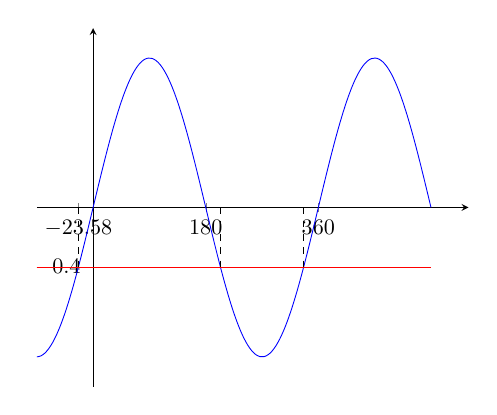
\begin{tikzpicture}[xscale=0.8, yscale=0.8]
    \begin{axis}[axis x line=middle, axis y line=middle, ymax=1.2, ymin=-1.2, xmax=600, xtick={-23.58, 0,180,360}, ytick={-0.4}]
        \addplot[
        smooth,
        color=blue,
        domain=-90:540,
        samples=100,
        ]{sin(x)};
        \addplot[
        color=red,
        domain=-90:540,
        ]{-0.4};
        \draw[dashed] (-23.58,0) -- (-23.58,-0.4);
        \draw[dashed] (203.58,0) -- (203.58,-0.4);
        \draw[dashed] (336.42,0) -- (336.42, -0.4);
    \end{axis}
    \end{tikzpicture}
\end{figure}

Using the calculator, $\sin^{-1}(-0.4)=-23.58^\circ$. From the graph, we see that the next value is $180+23.58 = 203.58^\circ$, and the next one $360-23.58 = 336.42^\circ$. Now let us look at the range of $y$ we need to find. The upper limit of $y$ is when $x=180^\circ$, i.e. $y=735^\circ$. So we also need the next few values of $y$, which is $360+203.58 = 563.58^\circ$ and $360+336.42=696.42^\circ$.

So overall our values of $y$ are $203.58,\,336.42,\,563.58,\,696.42$, or $x = 47.15,\,80.36,\,137.15,\,170.36$.

\iffalse

\textbf{Note:} There is a funny thing about the $\tan^{-1}$ in that for $x>0$,
\[
\tan^{-1}(x)+\tan^{-1}\left(\frac{1}{x}\right) = \frac{\pi}{2}\,.
\]
It is easiest to see this by drawing a right-angle triangle with short sides 1 and $x$.
\begin{figure}[H]
    \centering
    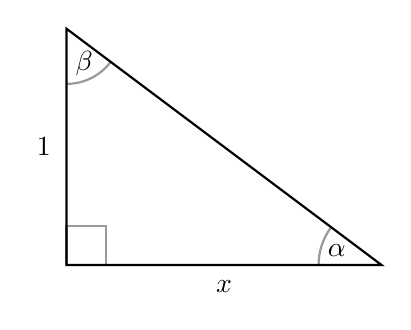
\begin{tikzpicture}[thick]
        \coordinate (O) at (0,0);
        \coordinate (A) at (4,0);
        \coordinate (B) at (0,3);
        \draw (O)--(A)--(B)--cycle;

        \tkzLabelSegment[below=2pt](O,A){$x$}
        \tkzLabelSegment[left=2pt](O,B){1}
        
        \tkzMarkAngle[fill=none,size=0.8cm, opacity=.4](B,A,O)
        \tkzLabelAngle[pos = 0.6](B,A,O){$\alpha$}
        \tkzMarkRightAngle[fill=none,size=0.5,opacity=.4](A,O,B)% square angle here

        \tkzMarkAngle[fill=none,size=0.7cm, opacity=.4](O,B,A)
        \tkzLabelAngle[pos = 0.5](O,B,A){$\beta$}
    \end{tikzpicture}
\end{figure}
Then $\alpha+\beta = 90^\circ$ with $\alpha = \tan^{-1}(1/x)$ and $\beta=\tan^{-1}x$.
\fi

\section{Angle addition}
When we have an equation with $\sin(x+a)$ and $\sin x$, where $a\neq 0$, we want to reduce it into an equation that only has $\sin x$ (or similarly with $\cos x$ or $\tan x$). \textbf{These are given in the formula booklet.}
\begin{align}
    \label{eqn:sinangle}
    \sin(\theta+\phi)&=\sin\theta\cos\phi+\cos\theta\sin\phi\\
    \label{eqn:cosangle}
    \cos(\theta+\phi)&=\cos\theta\cos\phi-\sin\theta\sin\phi\\
    \label{eqn:tanangle}
    \tan(\theta+\phi)&=\frac{\tan\theta+\tan\phi}{1-\tan\theta\tan\phi}
\end{align}

Equation \eqref{eqn:tanangle} is not used that often, since it gives a rather complicated result. It may be useful if we already know one of the angles.

If instead we have $\theta-\phi$, then simply substitute $\phi$ with $-\phi$ in equations \eqref{eqn:sinangle}--\eqref{eqn:tanangle} and use the property of $\sin$ and $\cos$ to get the right equation.

The double angle formula is when $\theta=\phi$. This gives a useful way of reducing e.g. $\sin4x$ into $\sin x$, or if we want to turn an equation with e.g. $\sin^4x$ into something with $\cos4x$, $\cos2x$ and $\cos x$. \textbf{These are not given in the formula booklet.} (You can easily derive them by setting the angles equal)
\begin{align}
    \sin2x&=2\sin x\cos x\\
    \label{eqn:cosdouble}
    \cos2x&=\cos^2x-\sin^2x = 2\cos^2x-1 = 1-2\sin^2x\\
    \tan2x&=\frac{2\tan x}{1-\tan^2x}
\end{align}

Equation \eqref{eqn:cosdouble} will be used a lot in cases like
\[
\int \sin^2x dx = \int\left(\frac{1}{2}-\frac{1}{2}\cos2x\right)dx = \frac{x}{2} - \frac{1}{4}\sin 2x
\]

\section{The ``$R$-formula"}
Usually in exams there will always be one part where they ask you to turn $a\cos\theta + b\sin\theta$ into something of the form $R\cos(\theta-\alpha)$ or $R\sin(\theta-\alpha)$, where $R$, $\alpha$ are constants, and $a$, $b$ are numbers that they give you. To do this, we simply apply the angle addition formula and equate the coefficients on the right hand side.

\textbf{Example.} Write $a\cos\theta + b\sin\theta$ as $R\sin(\theta+\alpha)$. Using \eqref{eqn:sinangle} and equating the two we have 
\begin{align}
    a\cos\theta + b\sin\theta&= R\sin(\theta+\alpha)\\
    &= \underbrace{R\cos\alpha}_{b}\sin\theta + \underbrace{R\sin\alpha}_a\cos\theta
\end{align}
so this gives $R\cos\alpha = b$, $R\sin\alpha=a$. Using \eqref{eqn:core} we get
\[
R^2=a^2+b^2\,,
\]
and dividing the two equations give
\[
\tan\alpha=\frac{a}{b}
\]

\textbf{Example.} Write $a\cos\theta+b\sin\theta$ as $R\cos(\theta-\alpha)$. Here we use \eqref{eqn:cosangle} and so we get
\begin{align}
    a\cos\theta + b\sin\theta&=R\cos(\theta-\alpha)\\
    &=R\cos\theta\cos\alpha + R\sin\theta\sin\alpha
\end{align}
so $R\cos\alpha = a$, $R\sin\alpha = b$. We get
\begin{align}
    R^2&=a^2+b^2\\
    \tan\alpha&=\frac{b}{a}\,.
\end{align}

\section{Other results}
These are not as often used as there aren't many cases where they actually simplify things. They can be all derived from the angle addition formulas. 
\begin{align}
    2\sin\theta\cos\phi = \sin(\theta+\phi) + \sin(\theta-\phi)\,,&\qquad 2\cos\theta\cos\phi = \cos(\theta+\phi) + \cos(\theta-\phi)\\
    2\cos\theta\sin\phi = \sin(\theta+\phi)-\sin(\theta-\phi)\,,&\qquad 2\sin\theta\sin\phi = -(\cos(\theta+\phi)-\cos(\theta-\phi))
\end{align}
These come from taking the following combinations, and are \textbf{not} given in the formula sheet.
\begin{align*}
    \sin(\theta+\phi) + \sin(\theta-\phi)&=\sin\theta\cos\phi+\cos\theta\sin\phi+\sin\theta\cos\phi-\cos\theta\sin\phi\\
    &=2\sin\theta\cos\phi\,,\\
    \cos(\theta+\phi)+\cos(\theta-\phi)&=\cos\theta\cos\phi -\sin\theta\sin\phi + \cos\theta\cos\phi+\sin\theta\sin\phi\\
    &= 2\cos\theta\cos\phi\,,\quad\text{and etc.}
\end{align*}
The following \textbf{are} given in the formula sheet, so you just need to know that they exist.
\begin{align}
    \sin\theta+\sin\phi=2\sin\left(\frac{\theta+\phi}{2}\right)\cos\left(\frac{\theta-\phi}{2}\right)\,,&\qquad\cos\theta+\cos\phi = 2\cos\left(\frac{\theta+\phi}{2}\right)\cos\left(\frac{\theta-\phi}{2}\right)\\
    \sin\theta-\sin\phi=2\sin\left(\frac{\theta-\phi}{2}\right)\cos\left(\frac{\theta+\phi}{2}\right)\,,&\qquad\cos\theta-\cos\phi=2\sin\left(\frac{\theta+\phi}{2}\right)\sin\left(\frac{\theta-\phi}{2}\right)
\end{align}
There aren't many cases where either sets of equations become useful, since they leave you with compound angles. The one exception is if e.g. $\theta=20x+10$, $\phi=18x+30$, then
\[
\cos(20x+10)+\cos(18x+30)=2\cos(19x+20)\cos(x-10)\,,
\]
which looks like
\begin{figure}[H]
    \centering
    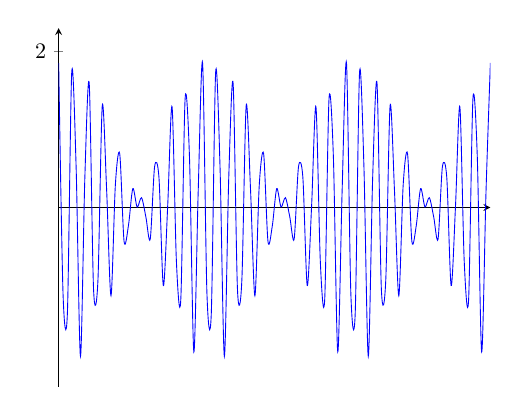
\begin{tikzpicture}[xscale=0.8, yscale=0.8]
    \begin{axis}[axis x line=middle, axis y line=middle, xticklabels=none, xtick={0}, ytick={2}, ymax=2.3, ymin=-2.3]
        \addplot[
        smooth,
        color=blue,
        domain=0:540,
        samples=100,
        ]{cos(20*x+10)+cos(18*x+30)};
    \end{axis}
    \end{tikzpicture}
\end{figure}


\end{document}
